\documentclass[a4paper, 12pt]{article}
\usepackage[utf8]{inputenc}
\setcounter{secnumdepth}{3} % para numerar los niveles de secciones, subsecciones, subsubsecciones
\usepackage[spanish,activeacute]{babel} % para establecer idioma
%\usepackage[english]{babel}
%\usepackage{cmbright} % para cambiar estilo de texto
\usepackage[T1]{fontenc}
\usepackage{fancyhdr}
\usepackage{calligra}
\usepackage{booktabs} % para tablas
%\usepackage{pythonhighlight}
%\PassOptionsToPackage{hyphens}{url}\usepackage[colorlinks=true,urlcolor=blue,citecolor=black,linkcolor=blue,hyperindex=true]{hyperref}
\PassOptionsToPackage{hyphens}{url}\usepackage[colorlinks=true,urlcolor=black,citecolor=black,linkcolor=black,hyperindex=true]{hyperref}
\usepackage[labelfont=bf]{caption}
\usepackage[section]{placeins}
\usepackage{textcomp}
\usepackage{acro}
\usepackage{amsmath}
\usepackage{amsthm}
\usepackage{amsfonts}
\usepackage{float}  % para forzar ubicacion de imagenes
\usepackage{pdflscape} % para cambiar orientación de pagina landscape
\usepackage[margin=1. in]{geometry} % Margenes
\usepackage{graphicx}
\graphicspath{ {files/} {chapters/chapter_1/images}}


\pagestyle{fancy}
\fancyhf{}
%\rhead{Share\LaTeX}
\fancyhead[C]{Universidad Nacional de la Patagonia San Juan Bosco \\Cátedra: Hormigón I}

\rfoot{\thepage}
\lfoot{Andrés Cintas}

\begin{document}
\begin{center}
\underline{\Large{T.P.N°7: Pandeo}}
\end{center}

\begin{enumerate}
\item Se tiene una columna compuesta por perfiles UPN de 35 cm x 60cm, donde se aplica
una carga de 1000 kN en el baricentro de la sección. La altura es de 5m y se
considera como condición de vínculo empotrado - articulado en el plano YZ y
empotrado libre en el plano XZ. Uno de los cordones está formado por 2UPN 160
(unidos por diagonales) y el otro por dos UPN 140 (unidos por diagonales). Ambos
cordones se encuentran unidos mediante diagonales y montantes como se indican en
el dibujo. El acero a utilizar es F-24. Se requiere:
\begin{itemize}
\item Verificar la columna, en caso de no ser así, redimensionar
\item Dimensionar los elementos de enlace
\end{itemize}

\begin{figure}[H]
\begin{center}
     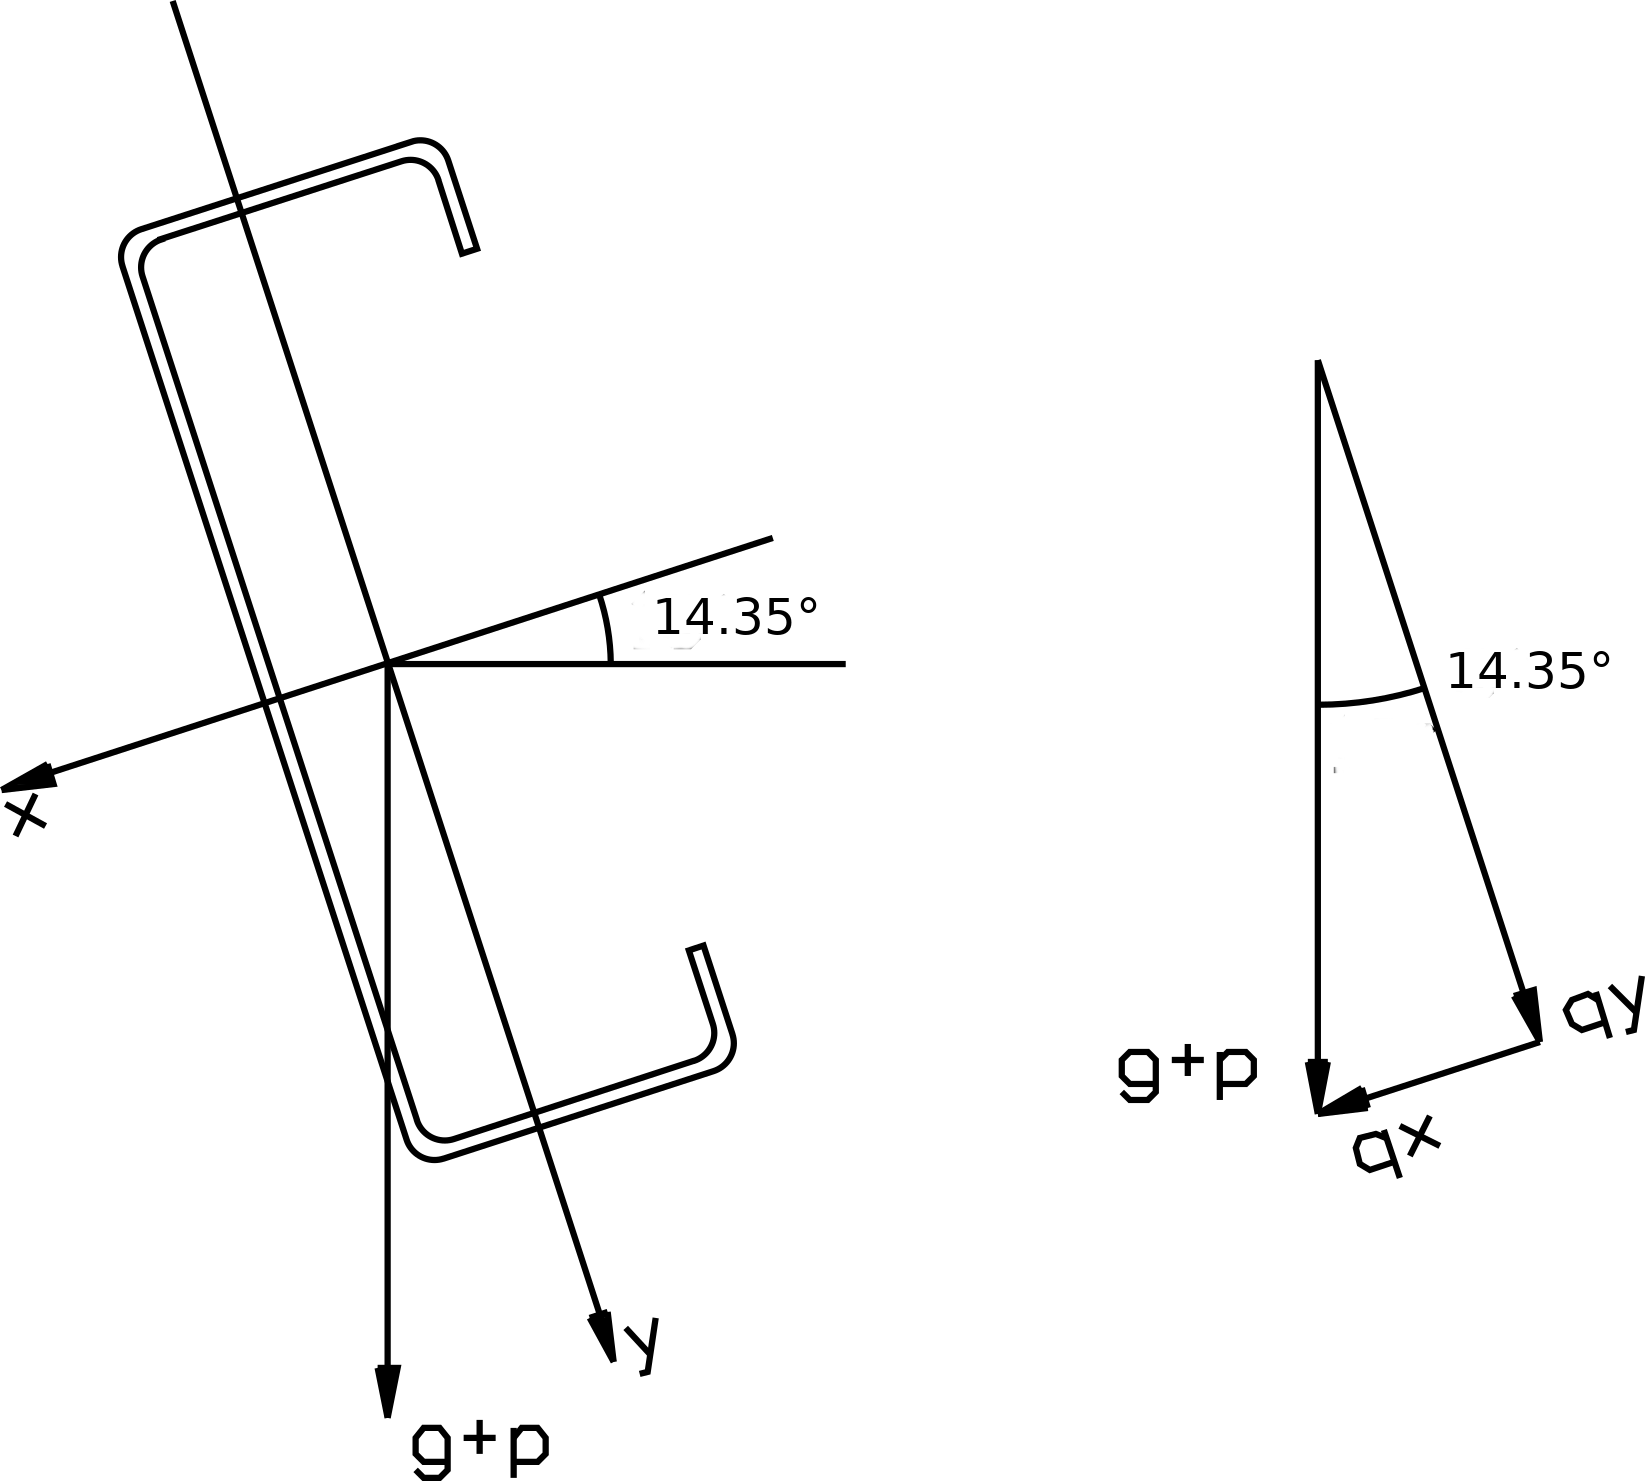
\includegraphics[scale = 1]{chapters/chapter_1/images/figura1.png}
\end{center}
\caption{Columna compuesta por perfiles UPN de 35 cm x 60cm}
\end{figure}
\item Determinar la carga ultima de una columna formada por 4 perfiles ángulos de 3 ½” x
½”. La altura es de 6m y se considera como condición de vínculo empotrado -
articulado en el plano YZ y empotrado libre en el plano XZ. La unión en el plano
YZ son mediante diagonales y la unión en el plano XZ son mediante diagonales y
montantes. El acero a utilizar es F-24. Dimensionar los elementos de enlaces.

\begin{figure}[H]
\begin{center}
     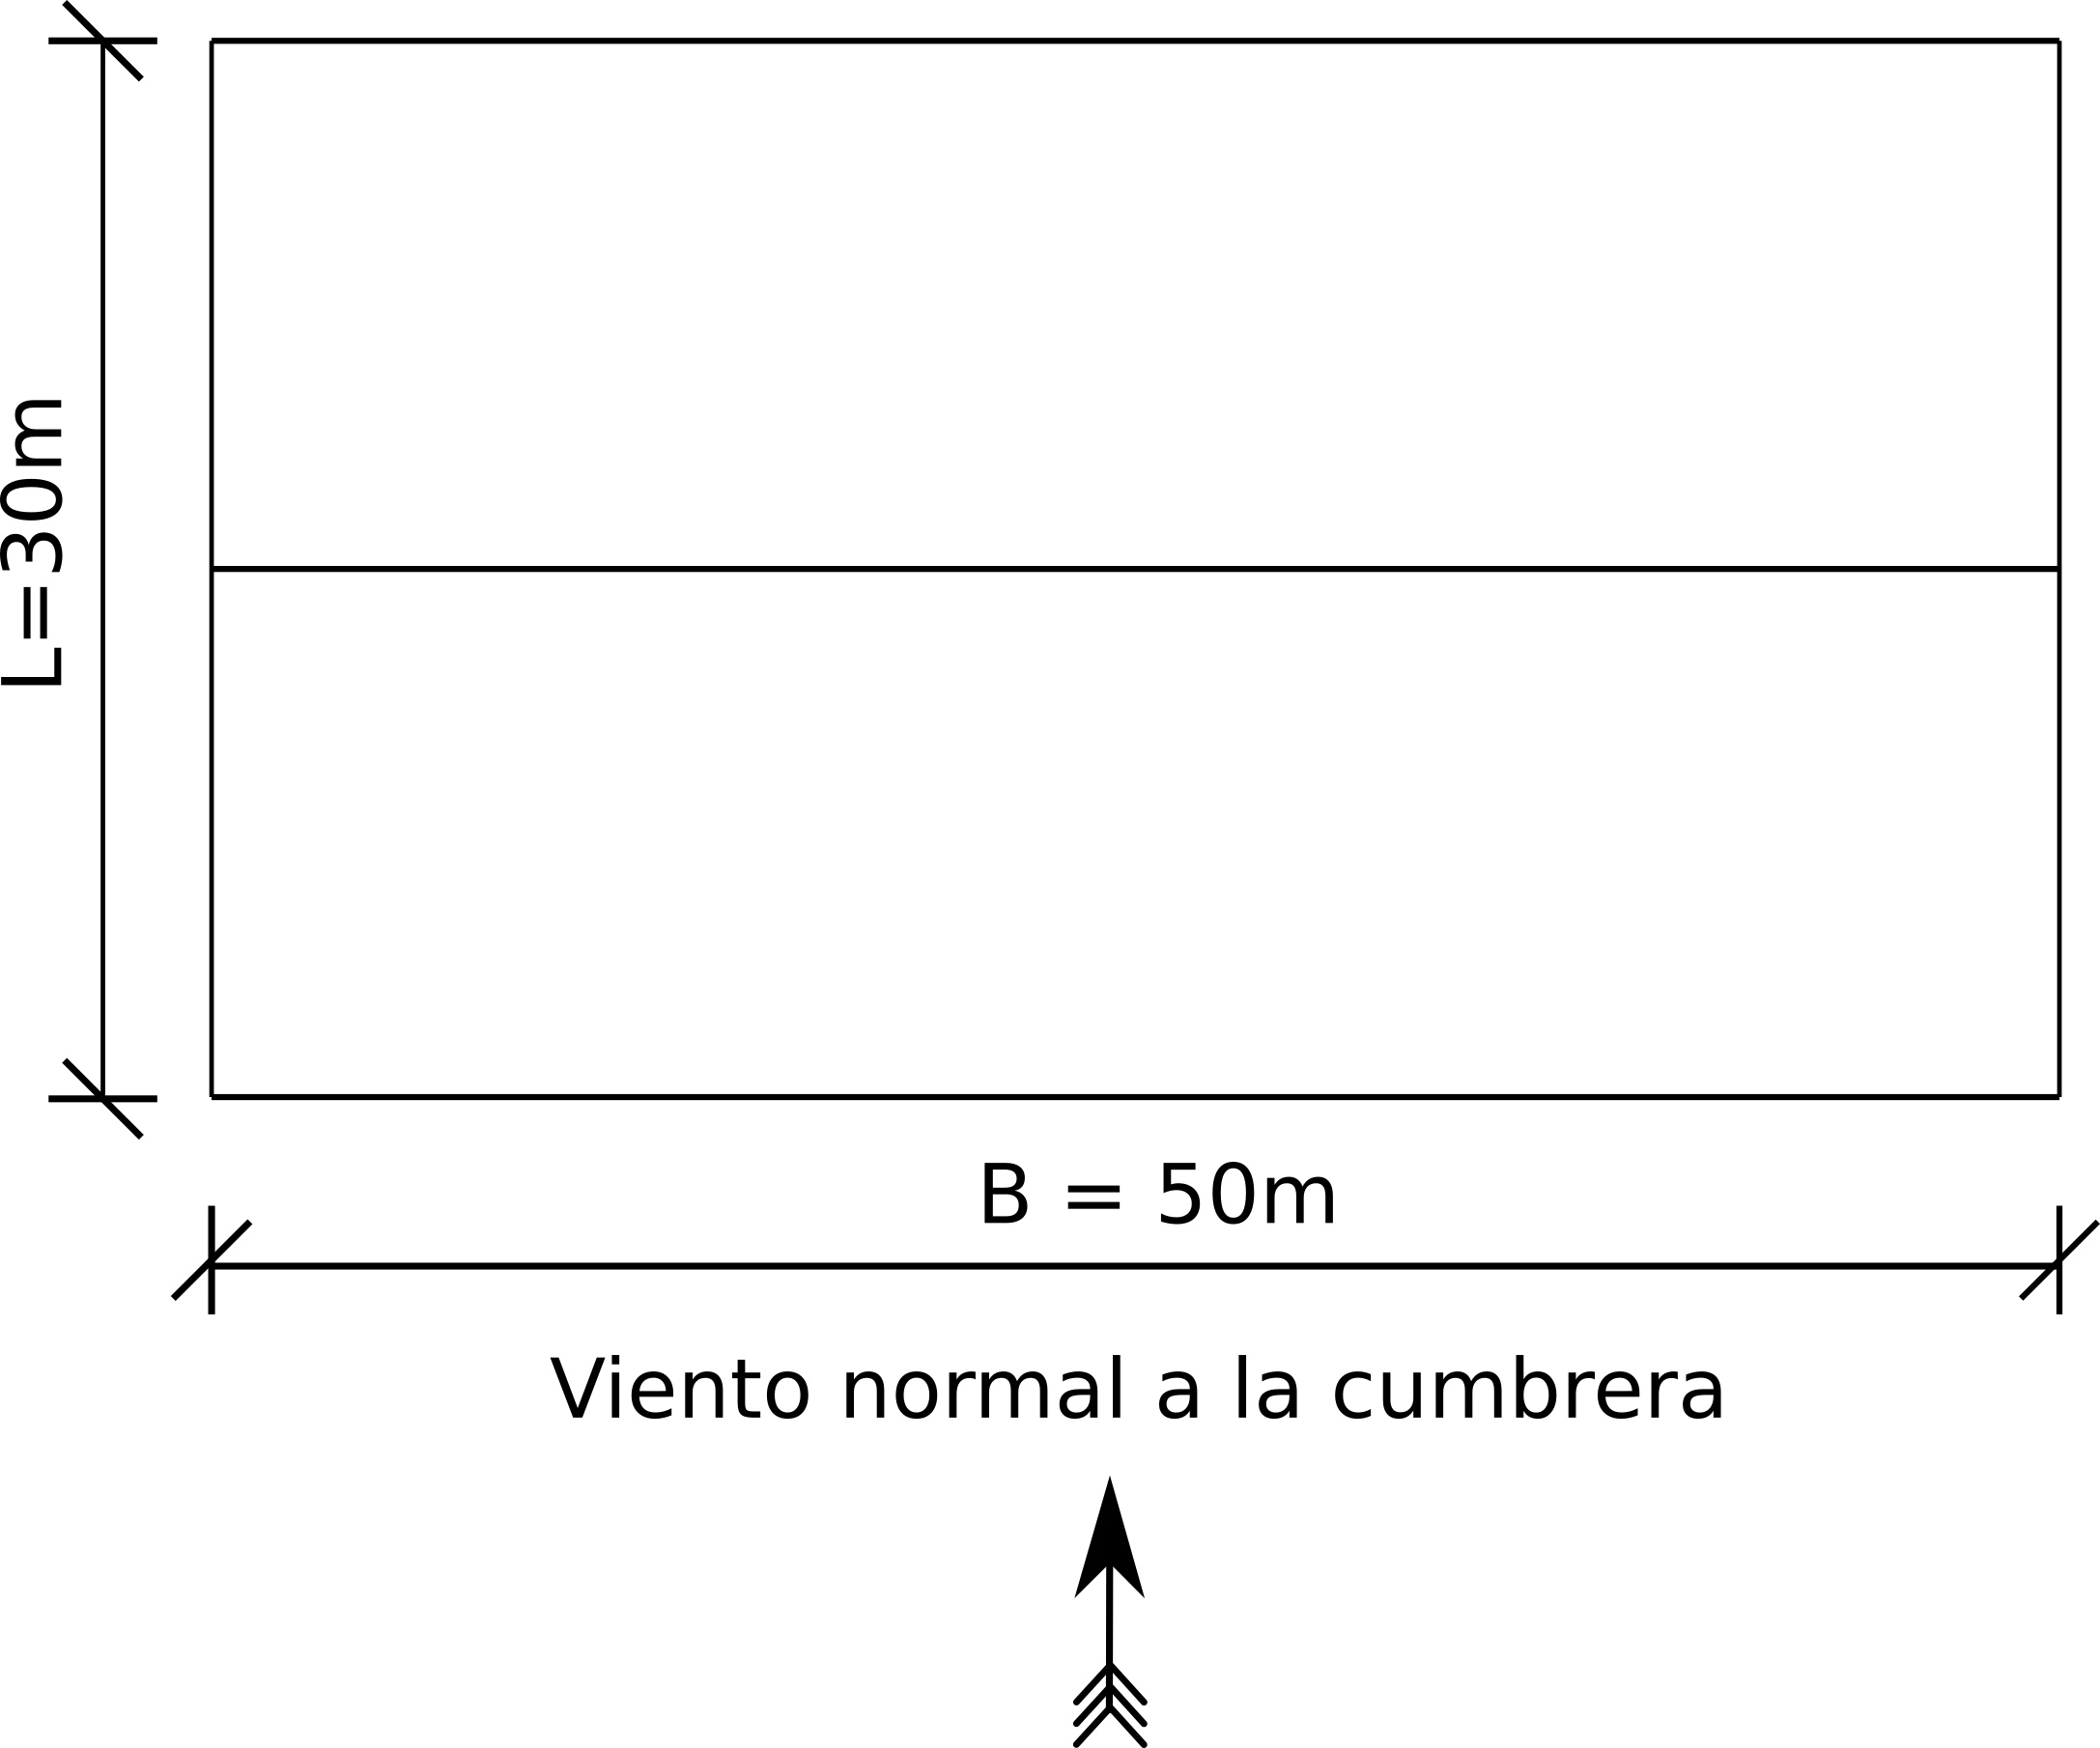
\includegraphics[scale = 1]{chapters/chapter_1/images/figura2.png}
\end{center}
\caption{Columna compuesta por perfiles L 3 ½” x 3 ½” x ½”}
\end{figure}
\end{enumerate}

\newpage

\begin{center}
\underline{\Large{Solución}}
\end{center}

\begin{enumerate}
\item Resolver una columna compuesta por perfiles UPN de 35 cm x 60cm.
\begin{itemize}
\item \underline{Datos}
\begin{align*}
& \text{Acero F-24}\\
& E = 200000MPa\\
& f_y = 235MPa\\
& P_u = 1000KN\\
& L = 500cm\\
& K_{yz} = 0.7\\
& K_{xz} = 2
\end{align*}
\begin{table}[H]
  \begin{center}
    \begin{tabular}{l|c|c} % <-- Alignments: 1st column left, 2nd middle and 3rd right, with vertical lines in between
      Perfil & UPN160 & UPN140\\
      \hline
      $I_x =$ & $925cm^4$ & $605cm^4$\\
      $I_y =$ & $85.3cm^4$ & $62.7cm^4$\\
      $r_x =$ & $6.21cm$ & $5.45cm$\\
      $r_y = r_1 =$ & $1.89cm$ & $1.75cm$\\
      $A_g =$ & $24cm^2$ & $20.4cm^2$\\
      $e_x =$ & $1.84cm$ & $1.75cm$\\
    \end{tabular}
  \end{center}
\end{table}

\begin{figure}[H]
\begin{center}
     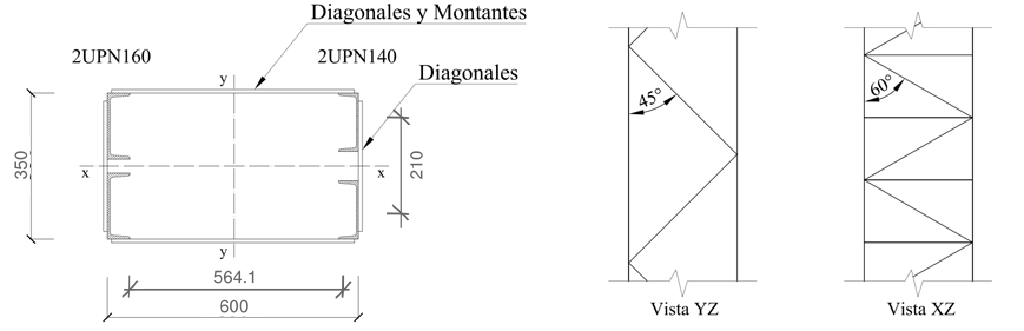
\includegraphics[scale = 1]{chapters/chapter_1/images/figura1_bis.png}
\end{center}
\caption{Columna compuesta por perfiles UPN de 35 cm x 60cm}
\end{figure}

\newpage
\item \underline{Eje libre x-x $\rightarrow$ Plano YZ}\\
Condición de sustentación empotrado-articulado $\Rightarrow K_{yz} = 0.70$

\item \underline{Momentos de Inercia y Radio de Giro}
\begin{align*}
& d_1 = \frac{35cm}{2} - 8cm = 9.5cm\\
& d_2 = \frac{35cm}{2} - 7cm = 10.5cm\\
& d_3 = \frac{60cm}{2} - e_x = \frac{60cm}{2} - 1.84cm = 28.16cm\\
& d_4 = \frac{60cm}{2} - e_x = \frac{60cm}{2} - 1.75cm = 28.25cm\\
& I_{xx} = [(I_{xx UPN160}+A_g \cdot d_1^2)+ (I_{xx UPN140}+A_g \cdot d_2^2)] \cdot 2\\
& I_{xx} = [(925cm^4+24cm^2 \cdot (9.5cm)^2)+ (605cm^4+20.4cm^2 \cdot (10.5cm)^2)] \cdot 2 = \framebox{$11890.2cm^4$}\\
& r_x = \sqrt{\frac{I_{xx}}{A_t}} = \sqrt{\frac{11890.2cm^4}{2\cdot(24cm^2 + 20.4cm^2)}} = \framebox{$11.57cm$}
\end{align*}

\item \underline{Esbeltez modificada}
\begin{align*}
& \lambda_0 = \frac{K_{yz} \cdot L}{r_x} = \frac{0.70 \cdot 500cm}{11.57cm} = \framebox{$30.25$}\\
& \lambda_0 < 200 \\
& 30.25 < 200 \quad \surd \quad \text{Verifica} \\
& \alpha = 45\text{°}\\
& h = 2 \cdot d_2 = 2 \cdot 10.5cm = \framebox{$21cm$} \\
& a = 2 \cdot \frac{h}{tg \alpha} = 2 \cdot \frac{21cm}{tg(45\text{°})} = \framebox{$42cm$}\\
& d = \frac{h}{Sen\alpha} = \frac{21cm}{Sen(45\text{°})} = \framebox{$29.70cm$}\\
& \text{Adopto diagonales de perfil L 1 ½” x 1 ½” x 3/16”} \\
& A_d = 3.46cm^2 \\
& r_1 = 0.72cm \\
& \lambda_1 = \pi \cdot \sqrt{\frac{2 \cdot A_g \cdot d^3}{n_0 \cdot A_d \cdot a \cdot h^2}} \\
& n_0 = \text{n° de planos de celosía = 2} \\
& \lambda_1 = \pi \cdot \sqrt{\frac{2 \cdot (2\cdot(24cm^2+20.4cm^2)) \cdot (29.70cm)^3}{2 \cdot 3.46cm^2 \cdot 42cm \cdot (21cm)^2}} = \framebox{$18.93$}\\
& \lambda_m = \sqrt{\lambda_0^2 + \lambda_1^2} = \sqrt{(30.25)^2 + (18.93)^2} = \framebox{$35.68$}
\end{align*}

\item \underline{Resistencia de diseño local}
\begin{align*}
& P_{cm} = \frac{\pi^2 \cdot E \cdot A_g}{\lambda_m^2} \cdot 10^{-1}\\
& P_{cm} = \frac{\pi^2 \cdot 200000MPa \cdot 2 \cdot (24cm^2+20.4cm^2)}{(35.68)^2} \cdot 10^{-1} = \framebox{$13768.38KN$}\\
& e_0 = \frac{K_{yz} \cdot L}{500} = \frac{0.70 \cdot 500cm}{500} = \framebox{$0.70cm$} \\
& M_s = \frac{P_u \cdot e_0}{1-\frac{P_u}{P_{cm}}} \cdot 10^{-2} = \frac{1000KN \cdot 0.70cm}{1-\frac{1000KN}{13768.38KN}} \cdot 10^{-2} = \framebox{$ 7.55KN.m$} \\
& P_{u1} = \frac{P_u}{n} + \frac{M_s}{n_1 \cdot h} \cdot 10^2 \\
& P_{u1} = \frac{1000KN}{4} + \frac{7.55KN.m}{2 \cdot 21cm} \cdot 10^2 = \framebox{$267.97KN$}\\
& n = \text{n° de barras de la columna armada} \Rightarrow 4 \\
& n_1 = \text{n° de barras que forman el cordón} \Rightarrow 2 \\
& \lambda_{c1} = \frac{1}{\pi} \cdot \frac{L_1}{r_1} \cdot \sqrt{\frac{f_y}{E}} \\
& L_1 = a = 42cm \\
& \lambda_{c1} = \frac{1}{\pi} \cdot \frac{42cm}{1.75cm} \cdot \sqrt{\frac{235MPa}{200000MPa}} = \framebox{$0.26$} \\
& \lambda_{c1} < 1.5 \\
& 0.26 < 1.5 \quad \surd \quad \text{Verifica} \\
& F_{cr} = 0.658^{\lambda_{c1}^2} \cdot f_y = 0.658^{0.26^2} \cdot 235MPa = \framebox{$228.35MPa$}\\
& P_{d1} = 0.85 \cdot F_{cr} \cdot A_g \cdot 10^{-1} = 0.85 \cdot 228.35MPa \cdot 20.40cm^2 \cdot 10^{-1} = \framebox{$395.96KN$} \\
& P_{d1} > P_{u1} \\
& 395.96KN > 267.97KN \quad \surd \quad \text{Verifica} \\
\end{align*}
\newpage
\item \underline{Verificación de las diagonales}

\begin{align*}
& \text{Corte } V_{eu} \\
& V_{eu} = \beta_1 \cdot P_u \\
& \beta_1 = \frac{\pi}{500} \cdot \Big[\frac{1}{1-\frac{P_u}{P_{cm}}} \Big] = \frac{\pi}{500} \cdot \Big[\frac{1}{1-\frac{1000KN}{13768.38KN}} \Big] = \framebox{$0.00678$}\\
& V_{eu} = 0.00678 \cdot 1000KN = \framebox{$6.78KN$} \\
& \text{El esfuerzo que solicita a la diagonal es } D_u \\
& D_u = \frac{V_{eu}}{2 \cdot Cos\alpha} = \frac{6.78KN}{2 \cdot Cos(45\text{°})} = \framebox{$4.79KN$} \\
& \text{La resistencia de diseño del perfil ángulo es } R_d \\
& R_d = \phi_c \cdot P_n \\
& R_d > D_u \\
& \text{Se determina el factor de esbeltez adimensional } \lambda_c \\
& \lambda_c = \frac{1}{\pi} \cdot \frac{K_{yz}\cdot L_1}{r_1} \cdot \sqrt{\frac{f_y}{E}} \\
& L_1 = d = 29.70cm \\
& \lambda_c = \frac{1}{\pi} \cdot \frac{0.70 \cdot 29.70cm}{0.72cm} \cdot \sqrt{\frac{235MPa}{200000MPa}} = \framebox{$0.32$} \\
& \lambda_c < 1.5 \\
& 0.32 < 1.5 \quad \surd \quad \text{Verifica} \\
& F_{cr} = 0.658^{\lambda_c^2} \cdot f_y = 0.658^{0.32^2} \cdot 235MPa = \framebox{$225.44MPa$}\\
& P_n = F_{cr} \cdot A_g \cdot 10^{-1} = 225.44MPa \cdot 20.40cm^2 \cdot 10^{-1} = \framebox{$78KN$} \\
& R_d = \phi_c \cdot P_n = 0.85 \cdot 78KN = \framebox{$66.30KN$} \\
& R_d > D_u \\
& 66.30KN > 4.79KN \quad \surd \quad \text{Verifica} \\
\end{align*}
%********************************************************************************************************
\newpage
\item \underline{Eje libre y-y $\rightarrow$ Plano XZ}\\
Condición de sustentación empotrado-libre $\Rightarrow K_{xz} = 2$

\item \underline{Momentos de Inercia y Radio de Giro}
\begin{align*}
& d_1 = \frac{35cm}{2} - 8cm = 9.5cm\\
& d_2 = \frac{35cm}{2} - 7cm = 10.5cm\\
& d_3 = \frac{60cm}{2} - e_x = \frac{60cm}{2} - 1.84cm = 28.16cm\\
& d_4 = \frac{60cm}{2} - e_x = \frac{60cm}{2} - 1.75cm = 28.25cm\\
& I_{yy} = [(I_{yy UPN160}+A_g \cdot d_3^2)+ (I_{yy UPN140}+A_g \cdot d_4^2)] \cdot 2\\
& I_{yy} = [(85.3cm^4+24cm^2 \cdot (28.16cm)^2)+ (62.7cm^4+20.4cm^2 \cdot (28.25cm)^2)] \cdot 2 \\
& I_{yy} = \framebox{$70920.25cm^4$}\\
& r_y = \sqrt{\frac{I_{yy}}{A_t}} = \sqrt{\frac{70920.25cm^4}{2\cdot(24cm^2 + 20.4cm^2)}} = \framebox{$28.26cm$}
\end{align*}

\item \underline{Esbeltez modificada}
\begin{align*}
& \lambda_0 = \frac{K_{xz} \cdot L}{r_y} = \frac{2 \cdot 500cm}{28.26cm} = \framebox{$35.39$}\\
& \lambda_0 < 200 \\
& 35.39 < 200 \quad \surd \quad \text{Verifica} \\
& \alpha = 60\text{°}\\
& h = d_3 + d_4 = 28.16cm + 28.25cm = \framebox{$56.41cm$} \\
& a = \frac{h}{tg \alpha} = \frac{56.41cm}{tg(60\text{°})} = \framebox{$32.57cm$}\\
& d = \frac{h}{Sen\alpha} = \frac{56.41cm}{Sen(60\text{°})} = \framebox{$65.14cm$}\\
& \text{Adopto diagonales de perfil L 2” x 2” x 3/16”} \\
& A_d = 4.72cm^2 \\
& r_1 = 0.97cm \\
& \lambda_1 = \pi \cdot \sqrt{\frac{A_g \cdot d^3}{n_0 \cdot A_d \cdot a \cdot h^2}} \\
& n_0 = \text{n° de planos de celosía = 2} \\
& \lambda_1 = \pi \cdot \sqrt{\frac{(2\cdot(24cm^2+20.4cm^2)) \cdot (65.14cm)^3}{2 \cdot 4.72cm^2 \cdot 32.57cm \cdot (56.41cm)^2}} = \framebox{$15.73$}\\
& \lambda_m = \sqrt{\lambda_0^2 + \lambda_1^2} = \sqrt{(35.39)^2 + (15.73)^2} = \framebox{$38.73$}
\end{align*}

\item \underline{Resistencia de diseño local}
\begin{align*}
& P_{cm} = \frac{\pi^2 \cdot E \cdot A_g}{\lambda_m^2} \cdot 10^{-1}\\
& P_{cm} = \frac{\pi^2 \cdot 200000MPa \cdot 2 \cdot (24cm^2+20.4cm^2)}{(38.73)^2} \cdot 10^{-1} = \framebox{$11688.05KN$}\\
& e_0 = \frac{K_{xz} \cdot L}{500} = \frac{2 \cdot 500cm}{500} = \framebox{$2cm$} \\
& M_s = \frac{P_u \cdot e_0}{1-\frac{P_u}{P_{cm}}} \cdot 10^{-2} = \frac{1000KN \cdot 2cm}{1-\frac{1000KN}{11688.05KN}} \cdot 10^{-2} = \framebox{$ 21.87KN.m$} \\
& P_{u1} = \frac{P_u}{n} + \frac{M_s}{n_1 \cdot h} \cdot 10^2 \\
& P_{u1} = \frac{1000KN}{4} + \frac{21.87KN.m}{2 \cdot 56.41cm} \cdot 10^2 = \framebox{$269.39KN$}\\
& n = \text{n° de barras de la columna armada} \Rightarrow 4 \\
& n_1 = \text{n° de barras que forman el cordón} \Rightarrow 2 \\
& \lambda_{c1} = \frac{1}{\pi} \cdot \frac{L_1}{r_1} \cdot \sqrt{\frac{f_y}{E}} \\
& L_1 = a = 32.57cm \\
& \lambda_{c1} = \frac{1}{\pi} \cdot \frac{32.57cm}{1.75cm} \cdot \sqrt{\frac{235MPa}{200000MPa}} = \framebox{$0.20$} \\
& \lambda_{c1} < 1.5 \\
& 0.20 < 1.5 \quad \surd \quad \text{Verifica} \\
& F_{cr} = 0.658^{\lambda_{c1}^2} \cdot f_y = 0.658^{0.20^2} \cdot 235MPa = \framebox{$230.98MPa$}\\
& P_{d1} = 0.85 \cdot F_{cr} \cdot A_g \cdot 10^{-1} = 0.85 \cdot 230.98MPa \cdot 20.40cm^2 \cdot 10^{-1} = \framebox{$400.52KN$} \\
& P_{d1} > P_{u1} \\
& 400.52KN > 269.39KN \quad \surd \quad \text{Verifica} \\
\end{align*}
\newpage
\item \underline{Verificación de las diagonales}

\begin{align*}
& \text{Corte } V_{eu} \\
& V_{eu} = \beta_1 \cdot P_u \\
& \beta_1 = \frac{\pi}{500} \cdot \Big[\frac{1}{1-\frac{P_u}{P_{cm}}} \Big] = \frac{\pi}{500} \cdot \Big[\frac{1}{1-\frac{1000KN}{11688.05KN}} \Big] = \framebox{$0.00687$}\\
& V_{eu} = 0.00687 \cdot 1000KN = \framebox{$6.87KN$} \\
& \text{El esfuerzo que solicita a la diagonal es } D_u \\
& D_u = \frac{V_{eu}}{2 \cdot Cos\alpha} = \frac{6.87KN}{2 \cdot Cos(60\text{°})} = \framebox{$6.87KN$} \\
& \text{La resistencia de diseño del perfil ángulo es } R_d \\
& R_d = \phi_c \cdot P_n \\
& R_d > D_u \\
& \text{Se determina el factor de esbeltez adimensional } \lambda_c \\
& \lambda_c = \frac{1}{\pi} \cdot \frac{K_{xz}\cdot L_1}{r_1} \cdot \sqrt{\frac{f_y}{E}} \\
& L_1 = d = 65.14cm \\
& \lambda_c = \frac{1}{\pi} \cdot \frac{2 \cdot 65.14cm}{0.97cm} \cdot \sqrt{\frac{235MPa}{200000MPa}} = \framebox{$1.47$} \\
& \lambda_c < 1.5 \\
& 1.47 < 1.5 \quad \surd \quad \text{Verifica} \\
& F_{cr} = 0.658^{\lambda_c^2} \cdot f_y = 0.658^{1.47^2} \cdot 235MPa = \framebox{$95.66MPa$}\\
& P_n = F_{cr} \cdot A_g \cdot 10^{-1} = 95.66MPa \cdot 20.40cm^2 \cdot 10^{-1} = \framebox{$45.15KN$} \\
& R_d = \phi_c \cdot P_n = 0.85 \cdot 45.15KN = \framebox{$38.38KN$} \\
& R_d > D_u \\
& 38.38KN > 4.79KN \quad \surd \quad \text{Verifica} \\
\end{align*}
\end{itemize}

\end{document}